  \textbf{Results on GPU and CPU load balance}: Fig.~\ref{figs:cpu-gpu-balance} 
  shows two time steps of the timeline of running DHFR using 4 CPU cores and 1 GPU. 
  In the first time step, all work is offload to GPU, which is the original design.
  The time cost for this step is $848 ms$. After applying the new balance scheme
  we discussed in section~\ref{sec:balance}, the time line is shown in the second step.
  We can see that all 4 CPU cores and the GPU is kept busy all the time. The time step 
  is $178 ms$, which is 4.8x speedup.
On Blue Waters, we achieved speedup of 1.3x due to the fast GPU.

\begin{figure}[h]
\centering
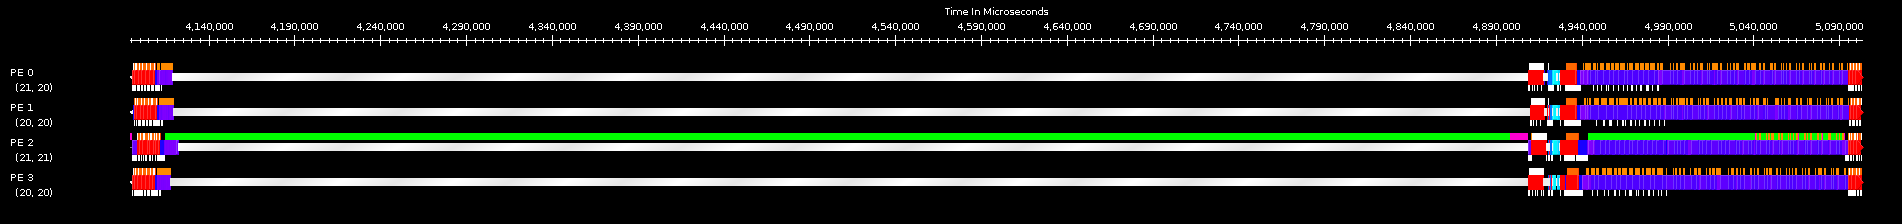
\includegraphics[width=6.5in]{figs/gpu-cpu-balance-timeline.png}
\caption{Timeline of running DHFR before and after load balance}
\label{figs:cpu-gpu-balance}
\end{figure}

\textbf{GPU kernel optimization results}: For tiling of patch 1 atoms, on the first
machine with GTX8800 GPU, we observed performance improvement as indicated in Fig.~\ref{figs:tile1-perf}.
The best performance improvement is 22\% when tile width is larger or equal to 4. Because the total
number of atoms in patch 1 is around 400, which takes 4 loops to be loaded and calculated on.
On JYC, we didn't see any improvement. With the help of profiling tools (``nvvp''), we found that after we increased tiling width for patch 1 atoms,
the amount of shared memory used by pairlist per thread is also rised. On this GPU, the occupancy is bounded by shared memory usage.
Therefore, increasing the total amount of shared memory usage leads to the decreasing of active thread blocks per SM.
As a result, the occupancy is reduced below 50\%, less than the original version.

However for GTX8800, the occupancy keeps the same for the cases of using tiling or not. This
is because its occupancy is bounded by register usage not shared memory usage, and we didn't change the number of registers per thread.
On the other hand, because GTX8800 is a quite old machine, the overhead of synchronization
divergence is more outstanding than JYC, therefore tiling of patch 1 atoms is able to improve its performance by reducing
synchronization latency.

\begin{figure}[h]
\centering
\setlength{\abovecaptionskip}{-1pt}
\setlength{\belowcaptionskip}{-2pt}
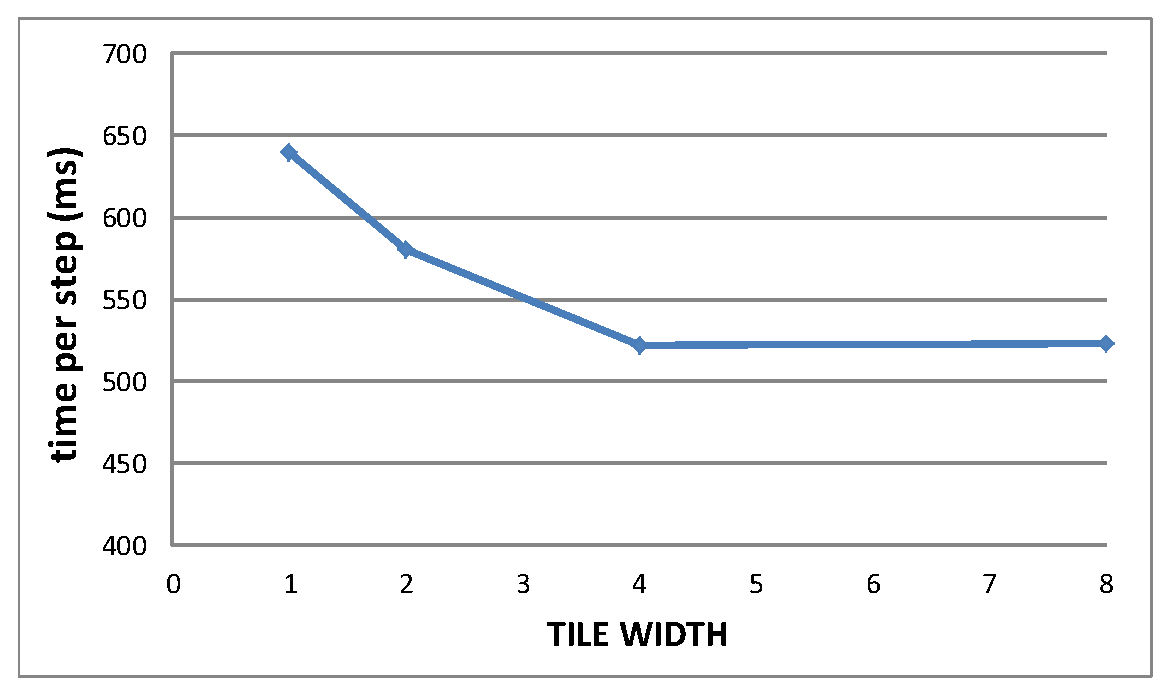
\includegraphics[width=4.0in]{figs/tile1-perf.eps}
\caption{Performance Improvement for tiling of patch 1 atoms}
\label{figs:tile1-perf}
%\vspace{-0.5cm}
\end{figure}

After implementing tiling of patch 2 atoms, we still didn't see performance improvement, because usage
of shared memory is continuing being increased and the occupancy is reduced. 

We also implemented the sorting strategy in the code, but didn't see any performance improvement. There are two
reasons for this: (1) after sorting, global memory access patterns for patch 1 atoms are not coalesced any more but become
very random, therefore overhead of load and store is increased. In other words, even though we make computation pattern regular
by sorting strategy, the memory access pattern becomes irregular. (2) Since we sort patch 1 atoms based on workload
on each atom, it makes sense when atoms in patch 2 are completely tiled. However, due to the shared memory
reason discussed above, tiling of patch 2 atoms makes performance worse, and it outweighs the benefit of sorting strategy.



